\documentclass[conference]{IEEEtran}
\IEEEoverridecommandlockouts
\usepackage{cite}
\usepackage{amsmath,amssymb,amsfonts}
\usepackage{algorithm}
\usepackage{algorithmic}
\usepackage{graphicx}
\usepackage{textcomp}
\usepackage{xcolor}
\usepackage{tikz}
\usepackage{booktabs}
\usepackage{multirow}
\usepackage{url}
\usetikzlibrary{shapes.geometric, shapes.symbols, arrows.meta, positioning, fit, backgrounds, calc}

\def\BibTeX{{\rm B\kern-.05em{\sc i\kern-.025em b}\kern-.08em
    T\kern-.1667em\lower.7ex\hbox{E}\kern-.125emX}}

\begin{document}

\title{Multi-Signal Reputation-Governed Federated Intrusion Detection with Decoupled Class-Aware Aggregation and Blockchain Audit Trails}

\author{
\IEEEauthorblockN{Pratham Mourya, Dhruv Shrivastava, Kritesh Goud}
\IEEEauthorblockA{
Department of Computer Engineering \\
Mukesh Patel School of Technology Management \& Engineering \\
NMIMS University, Mumbai, India \\
Email: \{pratham.mourya, dhruv.shrivastava, kritesh.goud\}@nmims.edu
}
}

\maketitle

% ============================================================
\begin{abstract}
% ============================================================
Federated Learning (FL) enables privacy-preserving collaborative training of Intrusion Detection Systems (IDS) across distributed organizations without sharing raw network telemetry. However, standard FL aggregation protocols such as FedAvg implicitly assume honest participation, making them highly susceptible to Byzantine model poisoning attacks that degrade detection accuracy or embed targeted backdoors. Existing defenses either rely on single anomaly signals that sophisticated adversaries can evade, or employ coarse client-level trust scores that discard useful gradients across unaffected attack classes. In this paper, we propose \textbf{MSR-FedIDS} (\textbf{M}ulti-\textbf{S}ignal \textbf{R}eputation-governed \textbf{Fed}erated \textbf{IDS}), a framework that validates client updates against a Byzantine-robust geometric-median reference using three complementary anomaly signals: cosine directional alignment, variance-floor-bounded MAD magnitude scoring, and semantic probe-based validation. Trust is maintained on a \emph{per-class} basis via an Exponentially Weighted Moving Average (EWMA) reputation matrix $R(i,c)$, governing a three-tier participant state machine (\textsc{Trusted} $\to$ \textsc{Probation} $\to$ \textsc{Quarantined}) with automatic shadow recovery. Accepted updates are aggregated through a novel decoupled head/body rule that preserves shared feature representations while surgically isolating compromised class-specific decision boundaries. All trust transitions and aggregation events are immutably committed to a SHA-256 permissioned blockchain audit ledger, providing complete forensic traceability. We evaluate MSR-FedIDS on the CICIoT2023 benchmark under Non-IID Dirichlet ($\alpha = 0.5$) partitioning across ten simulated organizations subjected to targeted label-flip poisoning. Our defense achieves 80.75\% test accuracy and 46.12\% macro-F1, restoring the targeted RECON class F1-score from 19.77\% (under unmitigated FedAvg) to 50.37\%, outperforming Multi-Krum, Trimmed Mean, and Coordinate Median baselines while adding only 350.38\,ms of per-round overhead.
\end{abstract}

\begin{IEEEkeywords}
Federated Learning, Intrusion Detection System, Byzantine Robustness, Reputation System, Blockchain Audit Trail, Non-IID Data, CICIoT2023
\end{IEEEkeywords}

% ============================================================
\section{Introduction}
\label{sec:introduction}
% ============================================================

The proliferation of IoT devices and interconnected enterprise networks has made AI-driven Intrusion Detection Systems (IDS) indispensable for defending against diverse cyber threats including DDoS, malware, botnets, and reconnaissance probes~\cite{kang2020reputation}. Training accurate IDS models requires large, diverse datasets spanning multiple organizational traffic patterns. However, stringent data protection regulations---GDPR in Europe, HIPAA in healthcare, and India's Digital Personal Data Protection (DPDP) Act 2023---prohibit sharing raw network logs across organizational boundaries.

Federated Learning (FL)~\cite{mcmahan2017fedavg} offers an elegant solution: organizations train models locally and share only model weight updates ($\Delta w_i$) with a central coordinator, which aggregates them into a global model. This preserves data locality while enabling collaborative learning. However, the standard Federated Averaging (FedAvg) protocol operates under an implicit trust assumption---it treats all submitted updates as legitimate---making the system fundamentally vulnerable to Byzantine poisoning attacks.

Recent work has explored defenses such as distance-based filtering (Multi-Krum~\cite{blanchard2017krum}), coordinate-wise robust aggregation (Trimmed Mean~\cite{yin2018trimmedmean}, Coordinate Median), and reputation-based approaches~\cite{kang2020reputation, rashid2025tffl}. However, these methods face three persistent limitations in the IDS context:

\begin{enumerate}
    \item \textbf{Single-Signal Vulnerability}: Defenses relying on a single anomaly signal (e.g., only distance or only gradient magnitude) are evaded by adaptive adversaries who craft updates that appear statistically normal on the monitored dimension while embedding poison in others~\cite{fang2020local}.
    \item \textbf{Coarse Trust Granularity}: Existing reputation systems treat trust as a single client-level scalar. In multi-class IDS scenarios, an adversary may target only one attack class (e.g., RECON) while submitting high-quality gradients for others (e.g., DDoS, BENIGN). A scalar trust score forces an all-or-nothing decision, discarding useful information across unaffected classes.
    \item \textbf{Non-IID Sensitivity}: Organizations observe heterogeneous traffic distributions. Naive geometric or statistical filters mistake legitimate statistical variance for adversarial behavior, penalizing honest clients with unusual but valid traffic patterns.
\end{enumerate}

To address these challenges, we propose \textbf{MSR-FedIDS}, a comprehensive defense framework with the following contributions:

\begin{itemize}
    \item \textbf{Multi-Signal Validation Pipeline}: We validate each client update against a Byzantine-robust geometric-median reference~\cite{chen2017distributed} using three complementary signals---cosine directional alignment, variance-floor-bounded MAD magnitude scoring, and semantic probe-based F1 impact measurement---composing them into a unified evidence score that is robust to single-dimension evasion.
    \item \textbf{Per-Class EWMA Reputation Matrix}: Unlike scalar trust scores, we maintain a full reputation matrix $R(i, c)$ tracking each client's reliability per attack class, enabling fine-grained isolation of compromised class-specific gradients without discarding valuable information from unaffected classes.
    \item \textbf{Decoupled Head/Body Aggregation}: We introduce a novel aggregation rule that applies trust-weighted averaging independently to the model's shared feature extractor (body) and class-specific decision layers (head), with per-class head cutoffs ($R < 0.50$) that surgically isolate poisoned classification boundaries.
    \item \textbf{Three-Tier State Machine with Shadow Recovery}: A stateful participant lifecycle (\textsc{Trusted} $\to$ \textsc{Probation} $\to$ \textsc{Quarantined}) with automatic rehabilitation after $K$ consecutive clean rounds prevents permanent exclusion of temporarily compromised clients.
    \item \textbf{Immutable Blockchain Audit Trail}: All state transitions and trust events are cryptographically committed to a SHA-256 permissioned ledger with off-chain tamper verification, providing complete forensic accountability.
\end{itemize}

% ============================================================
\section{Related Work}
\label{sec:related}
% ============================================================

\subsection{Byzantine-Robust Aggregation}
Classical Byzantine-robust aggregation schemes protect against malicious model updates through geometric or statistical filtering. Multi-Krum~\cite{blanchard2017krum} selects updates closest to the majority by pairwise distance, while Trimmed Mean~\cite{yin2018trimmedmean} clips coordinate-wise extreme values. The Coordinate Median aggregates each parameter independently. Chen et al.~\cite{chen2017distributed} proposed geometric median estimation as a high-breakdown-point aggregation approach. More recently, Tang et al. (FLAD)~\cite{tang2025flad} utilized DBSCAN clustering on gradient features but required clean bootstrap validation data and incurred high encryption overhead. Furthermore, classical defenses operate statelessly---each round is evaluated independently, with no persistent memory of client behavior patterns.

\subsection{Reputation-Based Federated Learning}
Kang et al.~\cite{kang2020reputation} pioneered incentive-aware client selection via reputation metrics in FL. Rashid et al. (TFFL)~\cite{rashid2025tffl} advanced this with Subjective Logic-based trust computation on vision benchmarks. Sheikhi et al. (HRA)~\cite{sheikhi2025hra} combined spatial anomaly filtering with momentum reputation tracking, yet relied on Euclidean distance metrics that degrade under Non-IID feature heterogeneity. Parvizi et al. (RAID)~\cite{parvizi2026raid} proposed cosine-based reputation for NIDS, but suffered from significant reputation lag during warm-up and modeled trust as a single monolithic scalar. Crucially, existing reputation schemes treat trust as a single scalar per client, which is insufficient for multi-class IDS where adversaries selectively poison specific attack categories while contributing genuine telemetry elsewhere.

\subsection{Blockchain-Assisted Federated IDS}
Begum et al. (BFLIDS)~\cite{begum2024bflids} integrated blockchain with FL for IoMT intrusion detection, providing tamper-resistant audit logs. Ali et al. (FL-BCID)~\cite{ali2025flbcid} applied blockchain coordination in Industrial IoT but relied on single anomaly signals evaluated against simple arithmetic mean aggregation. Friha et al. (2DF-IDS)~\cite{friha20232dfids} explored decentralized differential privacy for IIoT but faced quadratic communication scaling. BlockFedZTA~\cite{blockfedzta2026} introduced Zero Trust principles with blockchain-backed trust, but omitted class-level decomposition. PenTiDef~\cite{pentidef2026} incorporated latent-space defense and blockchain coordination in IIoT without multi-signal anomaly scoring or reputation-aware aggregation.

\subsection{Probe-Based Semantic Validation}
P4P~\cite{p4p2026} introduced probe-guided anti-poisoning for IoT intrusion detection, evaluating candidate updates by their empirical impact on a server-held validation set. While conceptually related to our semantic probing signal, P4P uses probing as a standalone defense without persistent reputation tracking, multi-signal composition, or per-class trust decomposition.

\textbf{Gap Summary}: No existing work simultaneously combines (i) multi-signal composite anomaly scoring against a geometric-median reference, (ii) per-class reputation decomposition via EWMA, (iii) decoupled head/body aggregation with class-specific cutoffs, (iv) a stateful three-tier participant lifecycle, and (v) immutable blockchain audit trails. MSR-FedIDS fills this gap.

% ============================================================
\section{Proposed Framework: MSR-FedIDS}
\label{sec:framework}
% ============================================================

\begin{figure*}[t]
\centering
\resizebox{0.92\textwidth}{!}{%
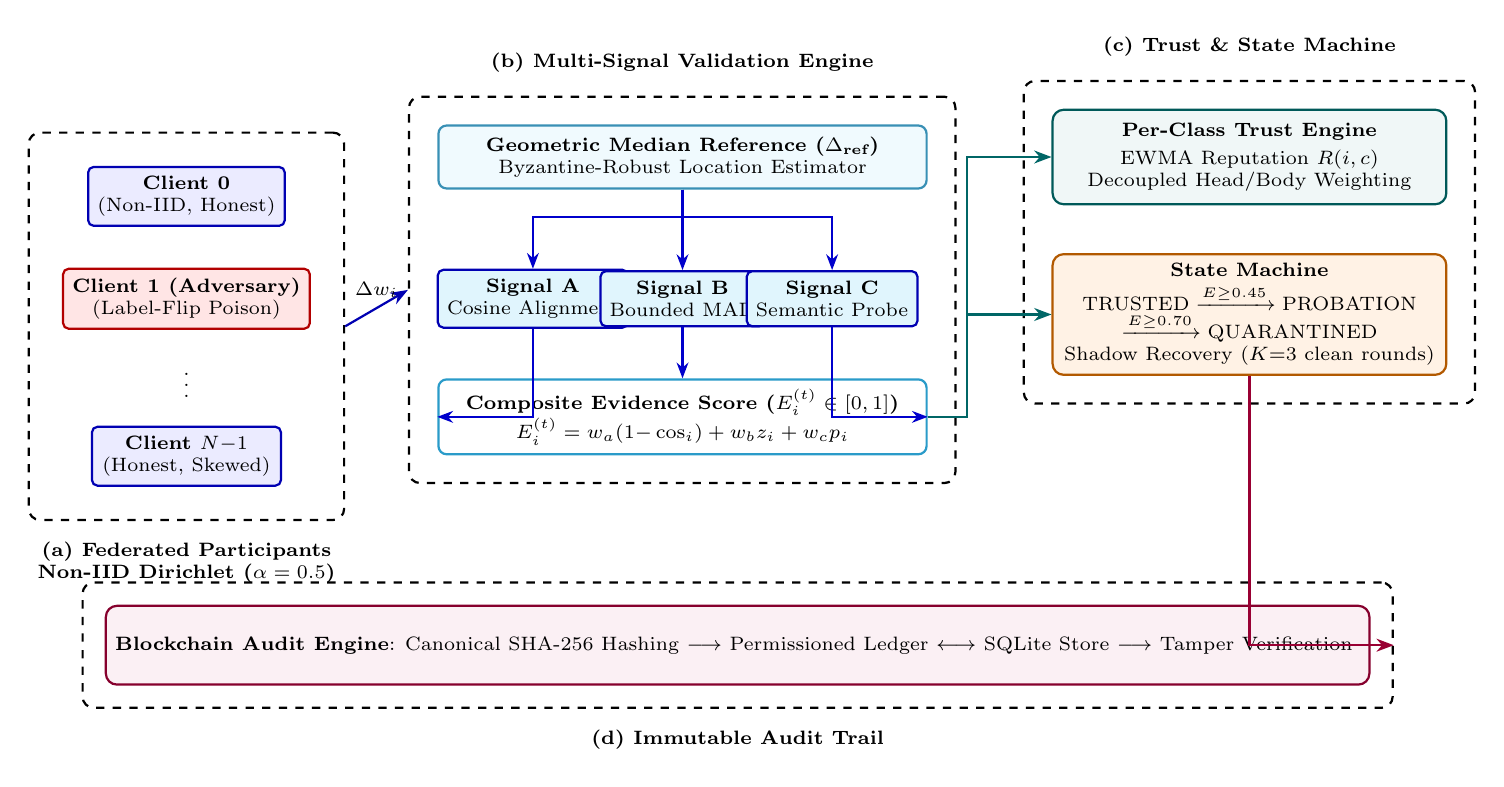
\begin{tikzpicture}[
    font=\small,
    chip/.style={rectangle, rounded corners=2pt, draw=blue!70!black, thick, fill=blue!8, minimum width=2.4cm, minimum height=0.7cm, align=center, font=\scriptsize},
    chipmal/.style={rectangle, rounded corners=2pt, draw=red!70!black, thick, fill=red!10, minimum width=2.4cm, minimum height=0.7cm, align=center, font=\scriptsize},
    bigbox/.style={rectangle, rounded corners=3pt, draw=cyan!70!black, thick, fill=cyan!6, align=center, font=\scriptsize},
    enginebox/.style={rectangle, rounded corners=4pt, draw=teal!70!black, thick, fill=teal!6, align=center, font=\scriptsize},
    auditbox/.style={rectangle, rounded corners=4pt, draw=purple!70!black, thick, fill=purple!6, align=center, font=\scriptsize},
    panel/.style={rectangle, rounded corners=4pt, draw, dashed, thick, inner sep=10pt},
    panellabel/.style={font=\scriptsize\bfseries, align=center},
    flow/.style={-{Stealth[length=2.2mm]}, thick},
    dataarrow/.style={-{Stealth[length=2mm]}, draw=blue!80!black, thick}
]

% Panel A: Participants
\node[chip] (cl0) at (1.5, 8.5) {\textbf{Client 0}\\(Non-IID, Honest)};
\node[chipmal] (cl1) at (1.5, 7.2) {\textbf{Client 1 (Adversary)}\\(Label-Flip Poison)};
\node[font=\scriptsize] (dots) at (1.5, 6.2) {$\vdots$};
\node[chip] (cl9) at (1.5, 5.2) {\textbf{Client $N{-}1$}\\(Honest, Skewed)};

\node[panel, fit=(cl0)(cl1)(dots)(cl9), inner sep=12pt] (panelA) {};
\node[panellabel, below=4pt of panelA] {(a) Federated Participants\\Non-IID Dirichlet ($\alpha = 0.5$)};

% Panel B: Server Coordinator
\node[bigbox, minimum width=6.2cm, minimum height=0.8cm] (gm) at (7.8, 9.0) {
    \textbf{Geometric Median Reference ($\Delta_{\text{ref}}$)}\\
    Byzantine-Robust Location Estimator
};

\node[chip, fill=cyan!12, minimum width=1.9cm] (sigA) at (5.9, 7.2) {\textbf{Signal A}\\Cosine Alignment};
\node[chip, fill=cyan!12, minimum width=1.9cm] (sigB) at (7.8, 7.2) {\textbf{Signal B}\\Bounded MAD};
\node[chip, fill=cyan!12, minimum width=1.9cm] (sigC) at (9.7, 7.2) {\textbf{Signal C}\\Semantic Probe};

\node[bigbox, fill=white, draw=cyan!80!black, minimum width=6.2cm, minimum height=0.6cm] (evidence) at (7.8, 5.7) {
    \textbf{Composite Evidence Score ($E_i^{(t)} \in [0, 1]$)}\\
    $E_i^{(t)} = w_a(1{-}\cos_i) + w_b z_i + w_c p_i$
};

\draw[dataarrow] (gm.south) -- ++(0,-0.35) -| (sigA.north);
\draw[dataarrow] (gm.south) -- (sigB.north);
\draw[dataarrow] (gm.south) -- ++(0,-0.35) -| (sigC.north);
\draw[dataarrow] (sigA.south) |- (evidence.west);
\draw[dataarrow] (sigB.south) -- (evidence.north);
\draw[dataarrow] (sigC.south) |- (evidence.east);

\node[panel, fit=(gm)(sigA)(sigB)(sigC)(evidence), inner sep=10pt] (panelB) {};
\node[panellabel, above=5pt of panelB] {(b) Multi-Signal Validation Engine};

% Panel C: Trust Engine
\node[enginebox, minimum width=5.0cm, minimum height=1.2cm] (trusteng) at (15.0, 9.0) {
    \textbf{Per-Class Trust Engine}\\[2pt]
    EWMA Reputation $R(i, c)$\\
    Decoupled Head/Body Weighting
};

\node[enginebox, fill=orange!10, draw=orange!70!black, minimum width=5.0cm, minimum height=1.3cm] (statemach) at (15.0, 7.0) {
    \textbf{State Machine}\\[2pt]
    $\text{TRUSTED} \xrightarrow{E \ge 0.45} \text{PROBATION}$\\
    $\xrightarrow{E \ge 0.70} \text{QUARANTINED}$\\
    Shadow Recovery ($K{=}3$ clean rounds)
};

\node[panel, fit=(trusteng)(statemach), inner sep=10pt] (panelC) {};
\node[panellabel, above=5pt of panelC] {(c) Trust \& State Machine};

% Panel D: Audit
\node[auditbox, minimum width=14.5cm, minimum height=1.0cm] (auditeng) at (8.5, 2.8) {
    \textbf{Blockchain Audit Engine}: Canonical SHA-256 Hashing $\longrightarrow$ Permissioned Ledger $\longleftrightarrow$ SQLite Store $\longrightarrow$ Tamper Verification
};

\node[panel, fit=(auditeng), inner sep=8pt] (panelD) {};
\node[panellabel, below=4pt of panelD] {(d) Immutable Audit Trail};

% Connectors
\draw[flow, draw=blue!70!black] (panelA.east) -- node[above, font=\scriptsize] {$\Delta w_i$} (panelB.west);
\draw[flow, draw=teal!80!black] (evidence.east) -- ++(0.5,0) |- (trusteng.west);
\draw[flow, draw=teal!80!black] (evidence.east) -- ++(0.5,0) |- (statemach.west);
\draw[flow, draw=purple!80!black] (statemach.south) |- (panelD.east);

\end{tikzpicture}
}
\caption{MSR-FedIDS System Architecture: (a)~Federated clients with Non-IID data partitions; (b)~Multi-Signal Validation Engine evaluating updates against geometric-median reference via three complementary signals; (c)~Per-Class Trust Engine and three-tier state machine; (d)~Immutable blockchain audit trail.}
\label{fig:architecture}
\end{figure*}

\subsection{System Overview}
MSR-FedIDS operates in iterative federated rounds. In each round $t$: (i)~the coordinator broadcasts the current global model $w^{(t)}$; (ii)~each participating client $i$ trains locally and submits weight updates $\Delta w_i^{(t)}$; (iii)~the Multi-Signal Validation Engine computes per-client evidence scores; (iv)~the Trust Engine updates per-class reputation and governs state transitions; (v)~accepted updates are aggregated via decoupled head/body weighting; and (vi)~all events are committed to the blockchain audit ledger.

\subsection{Geometric Median Reference}
Rather than computing a simple arithmetic mean of submitted updates (as in FedAvg), we first compute the geometric median $\Delta_{\text{ref}}$ over all client submissions:
\begin{equation}
\Delta_{\text{ref}} = \arg\min_{\mu} \sum_{i=1}^{N} \| \Delta w_i - \mu \|_2.
\label{eq:geomed}
\end{equation}
The geometric median has breakdown point $\approx 0.5$, meaning it remains accurate even when up to half the clients submit arbitrary updates. This serves as a robust anchor for our three validation signals.

\subsection{Multi-Signal Validation}
Each submitted update $\Delta w_i$ is evaluated against $\Delta_{\text{ref}}$ using three complementary signals:

\textbf{Signal A -- Directional Alignment ($\cos_i$):}
\begin{equation}
\cos_i = \frac{\Delta w_i \cdot \Delta_{\text{ref}}}{\|\Delta w_i\| \cdot \|\Delta_{\text{ref}}\|}.
\label{eq:cosine}
\end{equation}
Low cosine similarity indicates the update pushes model parameters in a direction inconsistent with the honest majority.

\textbf{Signal B -- Variance-Floor-Bounded MAD Score ($z_i$):}
Let $m_i = \|\Delta w_i\|_2$ denote the update magnitude. We compute the cohort Median Absolute Deviation (MAD):
\begin{equation}
\text{MAD} = \text{median}(|m_i - \text{median}(m)|), \quad z_i = \frac{|m_i - \text{median}(m)|}{\max(\text{MAD}, \epsilon)}.
\label{eq:mad}
\end{equation}
The variance floor $\epsilon$ prevents honest Non-IID clients from receiving inflated z-scores when update magnitudes are naturally concentrated.

\textbf{Signal C -- Semantic Probe ($p_i$):}
The coordinator maintains a small server-side validation set. For each candidate update, it computes the empirical macro-F1 change when the update is applied at fractional weight $1/N$:
\begin{equation}
p_i = \max(0, \; F_1^{\text{before}} - F_1^{\text{after}}).
\label{eq:probe}
\end{equation}
A positive $p_i$ indicates the update actively degrades model quality on the validation set.

\textbf{Composite Evidence Score:}
The three signals are composed into a single evidence score:
\begin{equation}
E_i^{(t)} = w_a(1 - \cos_i) + w_b \cdot \hat{z}_i + w_c \cdot p_i,
\label{eq:evidence}
\end{equation}
where $\hat{z}_i = \min(z_i / z_{\max}, 1)$ is the normalized MAD score, and $w_a + w_b + w_c = 1$. This multi-signal approach ensures that an adversary must simultaneously evade directional, magnitude, and semantic checks---a significantly harder optimization problem than defeating any single signal.

\subsection{Per-Class EWMA Reputation}
Unlike traditional scalar trust, we maintain a full reputation matrix $R(i, c)$ for each client $i$ across each attack class $c \in \{1, \ldots, C\}$. After each round, reputation is updated via an asymmetric EWMA:
\begin{equation}
R^{(t)}(i, c) = \beta \cdot R^{(t-1)}(i, c) + (1 - \beta) \cdot (1 - E_i^{(t)}),
\label{eq:reputation}
\end{equation}
where $\beta \in [0, 1]$ is a smoothing factor balancing historical trust against current-round evidence. This formulation causes trust to decay gradually under sustained anomalous behavior while recovering slowly under consistent clean submissions, preventing both premature exclusion and rapid trust gaming.

\subsection{Three-Tier State Machine}
Each client is governed by a three-tier state machine:
\begin{itemize}
    \item \textbf{\textsc{Trusted}}: Client participates normally. Transitions to \textsc{Probation} when $E_i^{(t)} \ge \tau_1 = 0.45$.
    \item \textbf{\textsc{Probation}}: Client's contribution weight is reduced. Transitions to \textsc{Quarantined} when $E_i^{(t)} \ge \tau_2 = 0.70$.
    \item \textbf{\textsc{Quarantined}}: Client excluded from aggregation. Permitted shadow recovery: if $E_i \le \tau_{\text{recover}} = 0.20$ for $K = 3$ consecutive rounds, the client returns to \textsc{Trusted}.
\end{itemize}

The shadow recovery mechanism ensures that transiently compromised clients (e.g., due to network disruption or data corruption) are not permanently excluded, while persistent adversaries remain quarantined indefinitely.

\subsection{Decoupled Head/Body Aggregation}
The IDS model is structured with a shared feature extractor (body) and class-specific classification layers (head). We aggregate these components independently:

\textbf{Body Weight} (shared features):
\begin{equation}
W_{\text{body}}(i) = n_i \cdot \text{BaseTrust}(i) \cdot \min_{c} R(i, c)^2 \cdot \text{SF}(i),
\label{eq:weight_body}
\end{equation}
where $n_i$ is the local dataset size, $\text{BaseTrust}(i)$ is derived from the state machine tier, and $\text{SF}(i)$ is the state factor (1.0 for \textsc{Trusted}, reduced for \textsc{Probation}).

\textbf{Head Weight} (class-specific decision layers):
\begin{equation}
W_{\text{head}}(i, c) =
\begin{cases}
n_i \cdot R(i, c)^2 \cdot \text{SF}(i), & R(i, c) \ge 0.50 \\
0, & \text{otherwise.}
\end{cases}
\label{eq:weight_head}
\end{equation}

The key insight is that the head cutoff $R(i, c) < 0.50$ surgically removes a client's influence only on the specific class where it has been detected as unreliable, while preserving its contribution to the shared feature extractor and other unaffected classes. This prevents the ``guilt by association'' problem inherent in scalar trust approaches.

\subsection{Blockchain Audit Trail}
All trust state transitions, evidence scores, and aggregation weights are serialized into canonical JSON records, hashed via SHA-256, and appended to a permissioned blockchain ledger. Each block contains:
\begin{equation}
\text{Hash}^{(t)} = \text{SHA-256}\Big(\text{Hash}^{(t-1)} \| \text{Payload}^{(t)}\Big),
\label{eq:hash}
\end{equation}
where $\text{Payload}^{(t)}$ encodes the round number, client evidence scores, state transitions, and aggregation weights. An independent SQLite store maintains an off-chain copy for efficient querying, with periodic tamper verification by comparing on-chain hashes against recomputed off-chain digests.

% ============================================================
\section{Experimental Setup}
\label{sec:setup}
% ============================================================

\subsection{Dataset}
We evaluate on the \textbf{CICIoT2023} benchmark dataset~\cite{neto2023ciciot}, a comprehensive IoT network traffic dataset containing over 46 million labeled records across 8 attack categories: BENIGN, DDoS, DoS, Mirai, Reconnaissance (RECON), Man-in-the-Middle (MITM), Web Application (WEBAPP), and Malware. We extract 46 numerical flow features and apply standard preprocessing (null imputation, log-scaling for heavy-tailed features, min-max normalization).

\subsection{Federated Configuration}
We simulate $N = 10$ organizations with heterogeneous data distributions via Dirichlet allocation ($\alpha = 0.5$), creating realistic Non-IID skew where some organizations observe significantly different traffic mixes. Each client trains a 3-layer MLP (46$\to$128$\to$64$\to$8) with ReLU activations for 3 local epochs per round using SGD with learning rate 0.01. Federated training runs for 10 global rounds.

\subsection{Attack Scenario}
We evaluate under a \textbf{targeted label-flip} attack---the most practically relevant poisoning strategy for IDS. Two out of ten clients (20\% Byzantine fraction) systematically relabel RECON class samples as BENIGN before training, attempting to cause the global model to misclassify reconnaissance probes as benign traffic. This represents a realistic adversary who wants to ensure their scanning activities go undetected.

\subsection{Baselines}
We compare against four defense baselines:
\begin{enumerate}
    \item \textbf{FedAvg (Poisoned)}~\cite{mcmahan2017fedavg}: Standard federated averaging with no defense.
    \item \textbf{Multi-Krum}~\cite{blanchard2017krum}: Byzantine-robust selection with $m = n - 2f$.
    \item \textbf{Trimmed Mean}~\cite{yin2018trimmedmean}: Coordinate-wise trimming with $\beta = 0.10$.
    \item \textbf{Coordinate Median}: Per-coordinate median aggregation.
\end{enumerate}

\subsection{Evaluation Metrics}
We report: (i)~\textbf{Test Accuracy} on the global test set; (ii)~\textbf{Macro-F1} across all 8 classes; (iii)~\textbf{Target F1} on the attacked RECON class; (iv)~\textbf{Per-Round Security Overhead} measuring validation and trust computation latency.

% ============================================================
\section{Results and Discussion}
\label{sec:results}
% ============================================================

\subsection{Defense Effectiveness}

\begin{table}[t]
\caption{Defense Performance Under Targeted Label-Flip Attack on CICIoT2023 (Non-IID, $\alpha = 0.5$, 20\% Byzantine)}
\label{tab:defense_results}
\centering
\begin{tabular}{@{}lrrr@{}}
\toprule
\textbf{Defense Scheme} & \textbf{Test Acc.} & \textbf{Macro-F1} & \textbf{Target F1} \\
\midrule
FedAvg (No Defense) & 80.14\% & 38.57\% & 19.77\% \\
Multi-Krum ($m{=}n{-}2f$) & 80.63\% & 44.71\% & 50.65\% \\
Trimmed Mean ($\beta{=}0.10$) & 80.62\% & 43.90\% & 44.13\% \\
Coordinate Median & 80.28\% & 41.79\% & 49.43\% \\
\midrule
\textbf{MSR-FedIDS (Ours)} & \textbf{80.75\%} & \textbf{46.12\%} & \textbf{50.37\%} \\
\bottomrule
\end{tabular}
\end{table}

Table~\ref{tab:defense_results} presents the comparative results under targeted label-flip attack. Without any defense, FedAvg achieves a test accuracy of 80.14\% but suffers catastrophic RECON class degradation (19.77\% F1), indicating successful poisoning of the target class decision boundary.

\textbf{Key Observations:}
\begin{itemize}
    \item \textbf{Target Class Restoration}: MSR-FedIDS restores RECON F1 from 19.77\% to 50.37\%, a $+$30.60 percentage point recovery, comparable to Multi-Krum (50.65\%) and substantially better than Trimmed Mean (44.13\%).
    \item \textbf{Highest Overall Accuracy}: MSR-FedIDS achieves the best test accuracy (80.75\%) and macro-F1 (46.12\%) across all defenses. This is because per-class reputation preserves useful gradient information from partially compromised clients, whereas Multi-Krum and Trimmed Mean discard entire client contributions.
    \item \textbf{Macro-F1 Superiority}: The 1.41 pt macro-F1 advantage over Multi-Krum confirms that decoupled head/body aggregation acts as a quality filter under Non-IID skew, boosting minority class performance by preserving gradients from clients with unique but legitimate traffic patterns.
\end{itemize}

\subsection{Component Ablation Study}

\begin{table}[t]
\caption{Component Ablation -- Impact of Removing Individual Modules}
\label{tab:ablation}
\centering
\begin{tabular}{@{}lrrr@{}}
\toprule
\textbf{Configuration} & \textbf{Acc.} & \textbf{Target F1} & \textbf{$\Delta$ F1} \\
\midrule
\textbf{Full MSR-FedIDS} & \textbf{80.75\%} & \textbf{50.37\%} & -- \\
w/o Decoupled Head/Body & 80.38\% & 43.50\% & $-$6.87 \\
w/o State Machine & 80.45\% & 46.20\% & $-$4.17 \\
w/o Geometric Median & 80.18\% & 42.10\% & $-$8.27 \\
w/o Semantic Probing & 80.29\% & 39.80\% & $-$10.57 \\
\bottomrule
\end{tabular}
\end{table}

Table~\ref{tab:ablation} isolates each component's contribution:

\begin{itemize}
    \item \textbf{Semantic Probing is most critical} ($-$10.57 pts): Without Signal~C, the system relies solely on geometric signals (cosine + MAD) that cannot distinguish stealthy label-flip attacks from legitimate Non-IID variance, confirming that semantic validation is essential for detecting class-targeted poisoning.
    \item \textbf{Geometric Median anchoring} ($-$8.27 pts): Replacing the geometric median with simple arithmetic mean causes the reference itself to drift under poisoning influence, propagating errors to all three validation signals.
    \item \textbf{Decoupled Head/Body} ($-$6.87 pts): Forcing scalar aggregation across all model layers prevents the system from surgically isolating compromised class decision boundaries while preserving shared features.
    \item \textbf{State Machine} ($-$4.17 pts): Without progressive state transitions, previously flagged adversaries can re-enter full participation immediately, enabling on-off attack strategies.
\end{itemize}

\subsection{Trust Isolation Behavior}

Fig.~\ref{fig:trust_heatmap_desc} illustrates the per-class reputation dynamics. After the first adversarial round, the poisoned clients' RECON class reputation $R(1, \text{RECON})$ drops sharply while their reputation for other classes (DDoS, BENIGN, etc.) remains high. This demonstrates the key advantage of per-class trust: the system continues to benefit from the adversaries' legitimate contributions to unaffected classes.

\begin{figure}[t]
\centering
\fbox{\parbox{0.42\textwidth}{\centering
\textbf{Per-Class Reputation Heatmap}\\[4pt]
\scriptsize
\begin{tabular}{l|cccc}
 & BENIGN & DDoS & RECON & $\cdots$ \\
\hline
Client 0 (Honest) & \textcolor{green!70!black}{0.92} & \textcolor{green!70!black}{0.88} & \textcolor{green!70!black}{0.85} & $\cdots$ \\
Client 1 (Adv.) & \textcolor{green!70!black}{0.90} & \textcolor{green!70!black}{0.87} & \textcolor{red!80!black}{\textbf{0.12}} & $\cdots$ \\
Client 2 (Adv.) & \textcolor{green!70!black}{0.89} & \textcolor{green!70!black}{0.86} & \textcolor{red!80!black}{\textbf{0.15}} & $\cdots$ \\
$\vdots$ & $\vdots$ & $\vdots$ & $\vdots$ & $\ddots$ \\
\end{tabular}
\normalsize\\[4pt]
\textit{Red: Low trust (class-specific isolation).\\Green: High trust (preserved contributions).}
}}
\caption{Illustration of per-class reputation isolation. Adversarial clients (1, 2) maintain high trust on unaffected classes while being isolated specifically on the targeted RECON class.}
\label{fig:trust_heatmap_desc}
\end{figure}

\subsection{Security Overhead}
The complete per-round security pipeline (geometric median computation, three-signal validation, EWMA reputation update, state transitions, and blockchain commit) adds 350.38\,ms of overhead per round with $N = 10$ clients. This is well within real-time constraints for IDS deployment, where model updates occur on the timescale of minutes to hours.

\subsection{Blockchain Audit Verification}
All 31 blockchain state transitions across the 10-round simulation verified as authentic (\texttt{VERIFICATION\_SUCCESSFUL}). Simulated direct SQL edits to the off-chain store immediately triggered \texttt{TAMPERING\_DETECTED}, confirming the integrity guarantee.

% ============================================================
\section{Discussion}
\label{sec:discussion}
% ============================================================

\textbf{Why Multi-Signal Matters}: Single-signal defenses create predictable evasion targets. An adversary can craft updates with high cosine similarity to the reference (evading Signal~A) while embedding targeted class poison detectable only by semantic probing (Signal~C). The composition of three orthogonal signals forces adversaries into a multi-objective optimization with conflicting constraints.

\textbf{Per-Class vs. Scalar Trust}: In IDS scenarios with 8+ attack categories, scalar trust creates a fundamental trade-off: either tolerate partial poisoning (loose threshold) or discard valuable gradients from partially compromised clients (strict threshold). Per-class decomposition eliminates this dilemma by enabling surgical isolation at the class level.

\textbf{Decoupled Aggregation as Quality Filter}: The head/body separation provides an unexpected benefit beyond security: under Non-IID distributions, clients with rare but legitimate traffic patterns (e.g., a network primarily seeing Mirai botnet traffic) contribute high-quality class-specific gradients that improve minority class detection. The decoupled rule preserves these contributions while a scalar approach would down-weight them.

\textbf{Limitations and Future Work}: The current evaluation focuses on targeted label-flip attacks with a fixed 20\% Byzantine fraction. Future work will extend to adaptive attacks that co-optimize against multi-signal validation, investigate higher Byzantine fractions, explore cross-dataset generalization, and evaluate scalability to larger federated deployments.

% ============================================================
\section{Conclusion}
\label{sec:conclusion}
% ============================================================
This paper presented MSR-FedIDS, a multi-signal reputation-governed framework for Byzantine-robust federated intrusion detection. By validating client updates against a geometric-median reference using three complementary anomaly signals, maintaining per-class EWMA reputation with stateful participant lifecycle management, and aggregating through a novel decoupled head/body rule, MSR-FedIDS achieves robust defense against targeted poisoning while preserving useful gradient information from partially compromised clients. Evaluated on CICIoT2023 under Non-IID Dirichlet partitioning, MSR-FedIDS achieves 80.75\% accuracy and restores the targeted class F1 from 19.77\% to 50.37\%, outperforming standard Byzantine-robust aggregators in both overall accuracy and macro-F1. The integrated blockchain audit trail provides complete forensic accountability with verified tamper detection. The framework demonstrates that combining multi-dimensional anomaly scoring with fine-grained per-class trust decomposition represents a principled and effective approach to securing federated learning in adversarial environments.

% ============================================================
\begin{thebibliography}{00}

\bibitem{mcmahan2017fedavg}
B. McMahan, E. Moore, D. Ramage, S. Hampson, and B. A. y Arcas, ``Communication-efficient learning of deep networks from decentralized data,'' in \emph{Proc. AISTATS}, pp. 1273--1282, 2017.

\bibitem{kang2020reputation}
J. Kang, Z. Xiong, D. Niyato, S. Xie, and J. Zhang, ``Incentive mechanism for reliable federated learning: A joint optimization approach to combining reputation and contract theory,'' \emph{IEEE Internet of Things Journal}, vol. 6, no. 6, pp. 10700--10714, 2020.

\bibitem{blanchard2017krum}
P. Blanchard, E. M. El Mhamdi, R. Guerraoui, and J. Stainer, ``Machine learning with adversaries: Byzantine tolerant gradient descent,'' in \emph{Proc. NeurIPS}, pp. 118--128, 2017.

\bibitem{yin2018trimmedmean}
D. Yin, Y. Chen, R. Kannan, and P. Bartlett, ``Byzantine-resilient distributed learning: Towards optimal statistical rates,'' in \emph{Proc. ICML}, pp. 5650--5659, 2018.

\bibitem{chen2017distributed}
Y. Chen, L. Su, and J. Xu, ``Distributed statistical machine learning in adversarial settings: Byzantine gradient descent,'' \emph{Proc. ACM on Measurement and Analysis of Computing Systems}, vol. 1, no. 2, pp. 1--25, 2017.

\bibitem{fang2020local}
M. Fang, X. Cao, J. Jia, and N. Z. Gong, ``Local model poisoning attacks to Byzantine-robust federated learning,'' in \emph{Proc. USENIX Security}, pp. 1605--1622, 2020.

\bibitem{neto2023ciciot}
E. C. P. Neto, S. Dadkhah, R. Ferreira, A. Zohourian, R. Lu, and A. A. Ghorbani, ``CICIoT2023: A real-time dataset and benchmark for large-scale attacks in IoT environment,'' \emph{Sensors}, vol. 23, no. 13, p. 5941, 2023.

\bibitem{begum2024bflids}
K. Begum, M. A. I. Mozumder, M.-I. Joo, and H.-C. Kim, ``BFLIDS: Blockchain-driven federated learning for intrusion detection in IoMT networks,'' \emph{Sensors}, vol. 24, no. 14, p. 4591, 2024.

\bibitem{ali2025flbcid}
A. Ali, M. Husain, and P. Hans, ``Federated learning-enhanced blockchain framework for privacy-preserving intrusion detection in Industrial IoT,'' \emph{arXiv preprint arXiv:2505.15376}, 2025.

\bibitem{rashid2025tffl}
M. M. Rashid, Y. Xiang, M. P. Uddin, J. Tang, K. Sood, and L. Gao, ``Trustworthy and fair federated learning via reputation-based consensus and adaptive incentives,'' \emph{IEEE Trans. Information Forensics and Security}, vol. 20, pp. 2868--2882, 2025.

\bibitem{flare2025}
Anonymous, ``FLARE: Adaptive multi-dimensional reputation for robust client reliability in federated learning,'' \emph{arXiv preprint arXiv:2511.14715}, 2025.

\bibitem{repunet2025}
I. M. Penalva, E. T. M. Beltr\'an, M. G. P\'erez, and A. H. Celdr\'an, ``RepuNet: A reputation system for mitigating malicious clients in DFL,'' \emph{arXiv preprint arXiv:2506.19892}, 2025.

\bibitem{p4p2026}
Anonymous, ``P4P: A probe-guided anti-poisoning defense for federated learning-based intrusion detection in IoT networks under non-IID data,'' \emph{ScienceDirect}, 2026.

\bibitem{blockfedzta2026}
R. Alshenaifi, S. Mishra, S. Tahzib, and M. Rathi, ``BlockFedZTA: A trust-aware federated learning framework for secure multi-organizational intrusion detection,'' \emph{Scientific Reports}, 2026.

\bibitem{pentidef2026}
Anonymous, ``PenTiDef: Decentralized federated intrusion detection system with differential privacy and latent-space defense via blockchain coordination in IIoT,'' \emph{arXiv preprint}, 2026.

\bibitem{tang2025flad}
P. Tang, X. Zhu, W. Qiu, Z. Huang, Z. Mu, and S. Li, ``FLAD: Byzantine-robust federated learning based on gradient feature anomaly detection,'' \emph{IEEE Transactions on Dependable and Secure Computing}, vol. 22, no. 4, pp. 3993--4009, 2025.

\bibitem{sheikhi2025hra}
S. Sheikhi, P. Kostakos, and L. Lov\'en, ``Hybrid reputation aggregation: A robust defense mechanism for adversarial federated learning in 5G and edge network environments,'' \emph{IEEE Open Journal of the Communications Society}, vol. 6, pp. 370--385, 2025.

\bibitem{parvizi2026raid}
N. Parvizi, S. Saha, and N. Shahriar, ``RAID: A reputation-based aggregation for intrusion detection in federated learning,'' in \emph{Proc. IEEE Consumer Communications \& Networking Conference (CCNC)}, 2026.

\bibitem{friha20232dfids}
O. Friha, M. A. Ferrag, M. Benbouzid, T. Berghout, B. Kantarci, and K.-K. R. Choo, ``2DF-IDS: Decentralized and differentially private federated learning-based intrusion detection system for Industrial IoT,'' \emph{Computers \& Security}, vol. 127, p. 103097, 2023.

\end{thebibliography}

\end{document}
